\begin{figure}[ht!]
    \centering
    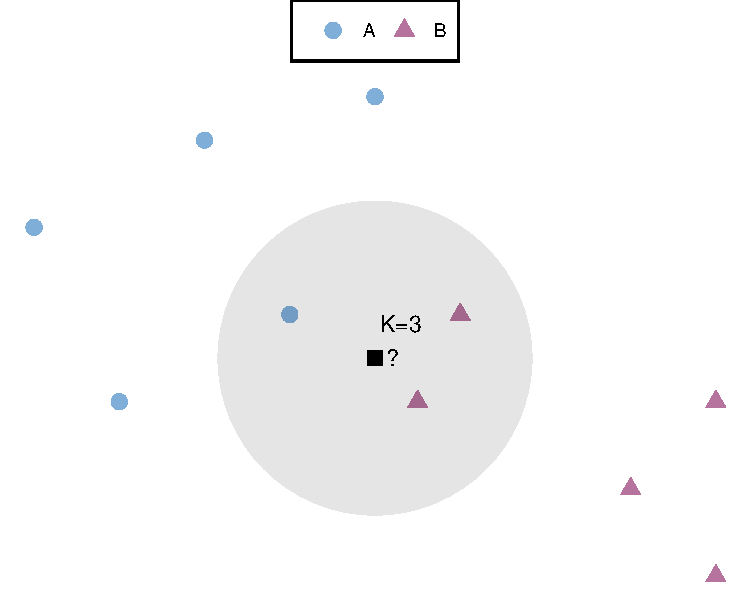
\includegraphics[scale=0.8]{graphics/knn_demo.pdf}
    \caption{\textbf{Illustration of K-nearest neighbours (KNN) algorithm.} When K=3, 3 neighbours to the new donor are identified based on the pre-calculated distances. The 3 neighbours get to ``vote'' for the prediction made on the new donor. Because there are 2 B's and 1 A, the new donor has cancer B.}
    \label{fig:knn_demo}
\end{figure}
